% Options for packages loaded elsewhere
\PassOptionsToPackage{unicode}{hyperref}
\PassOptionsToPackage{hyphens}{url}
\PassOptionsToPackage{dvipsnames,svgnames,x11names}{xcolor}
%
\documentclass[
]{article}
\usepackage{amsmath,amssymb}
\usepackage{iftex}
\ifPDFTeX
  \usepackage[T1]{fontenc}
  \usepackage[utf8]{inputenc}
  \usepackage{textcomp} % provide euro and other symbols
\else % if luatex or xetex
  \usepackage{unicode-math} % this also loads fontspec
  \defaultfontfeatures{Scale=MatchLowercase}
  \defaultfontfeatures[\rmfamily]{Ligatures=TeX,Scale=1}
\fi
\usepackage{lmodern}
\ifPDFTeX\else
  % xetex/luatex font selection
\fi
% Use upquote if available, for straight quotes in verbatim environments
\IfFileExists{upquote.sty}{\usepackage{upquote}}{}
\IfFileExists{microtype.sty}{% use microtype if available
  \usepackage[]{microtype}
  \UseMicrotypeSet[protrusion]{basicmath} % disable protrusion for tt fonts
}{}
\makeatletter
\@ifundefined{KOMAClassName}{% if non-KOMA class
  \IfFileExists{parskip.sty}{%
    \usepackage{parskip}
  }{% else
    \setlength{\parindent}{0pt}
    \setlength{\parskip}{6pt plus 2pt minus 1pt}}
}{% if KOMA class
  \KOMAoptions{parskip=half}}
\makeatother
\usepackage{xcolor}
\usepackage[margin=1in]{geometry}
\usepackage{longtable,booktabs,array}
\usepackage{calc} % for calculating minipage widths
% Correct order of tables after \paragraph or \subparagraph
\usepackage{etoolbox}
\makeatletter
\patchcmd\longtable{\par}{\if@noskipsec\mbox{}\fi\par}{}{}
\makeatother
% Allow footnotes in longtable head/foot
\IfFileExists{footnotehyper.sty}{\usepackage{footnotehyper}}{\usepackage{footnote}}
\makesavenoteenv{longtable}
\usepackage{graphicx}
\makeatletter
\def\maxwidth{\ifdim\Gin@nat@width>\linewidth\linewidth\else\Gin@nat@width\fi}
\def\maxheight{\ifdim\Gin@nat@height>\textheight\textheight\else\Gin@nat@height\fi}
\makeatother
% Scale images if necessary, so that they will not overflow the page
% margins by default, and it is still possible to overwrite the defaults
% using explicit options in \includegraphics[width, height, ...]{}
\setkeys{Gin}{width=\maxwidth,height=\maxheight,keepaspectratio}
% Set default figure placement to htbp
\makeatletter
\def\fps@figure{htbp}
\makeatother
\setlength{\emergencystretch}{3em} % prevent overfull lines
\providecommand{\tightlist}{%
  \setlength{\itemsep}{0pt}\setlength{\parskip}{0pt}}
\setcounter{secnumdepth}{-\maxdimen} % remove section numbering
\usepackage{fancyhdr}
\pagestyle{fancy}
\fancyhf{}
\lfoot[\thepage]{}
\rfoot[]{\thepage}
\fontsize{12}{22}
\selectfont
\usepackage{booktabs}
\usepackage{longtable}
\usepackage{array}
\usepackage{multirow}
\usepackage{wrapfig}
\usepackage{float}
\usepackage{colortbl}
\usepackage{pdflscape}
\usepackage{tabu}
\usepackage{threeparttable}
\usepackage{threeparttablex}
\usepackage[normalem]{ulem}
\usepackage{makecell}
\usepackage{xcolor}
\ifLuaTeX
  \usepackage{selnolig}  % disable illegal ligatures
\fi
\IfFileExists{bookmark.sty}{\usepackage{bookmark}}{\usepackage{hyperref}}
\IfFileExists{xurl.sty}{\usepackage{xurl}}{} % add URL line breaks if available
\urlstyle{same}
\hypersetup{
  colorlinks=true,
  linkcolor={blue},
  filecolor={Maroon},
  citecolor={Blue},
  urlcolor={Blue},
  pdfcreator={LaTeX via pandoc}}

\title{
\includegraphics[width=10cm,height=\textheight]{IEO-logo2.png}}
\author{}
\date{\vspace{-2.5em}}

\begin{document}
\maketitle


\pagenumbering{gobble}

%\begin{titlepage}
\begin{flushleft}
\Large{\textbf{Habitats Cadiz Gulf}}\\
\vspace*{2\baselineskip}
\LARGE{\textbf{Implementación metodológica SAR en pesquería de chirla \textit{Chamelea galllina} en el Golfo de Cádiz, España}}\\
\vspace*{5\baselineskip}
\Large{Grupo de Trabajo FEMP 04}\\
\vspace*{1\baselineskip}
\Large{Instituto Español de Oceanografía, Cádiz }\\
\vspace*{4\baselineskip}
\end{flushleft}
\begin{flushright}
\large{\textit{Mauricio Mardones}}\\
\large{\textit{Ana Magro}}\\
\vspace*{1\baselineskip}
\normalsize{\textbf{Fecha}}\\
Abril, 2024
\end{flushright}

% \end{titlepage}


\hypersetup{linkcolor = black}
\newpage
\pagenumbering{roman}
%\tableofcontents
%\addcontentsline{toc}{section}{\contentsname}

\newpage



\pagenumbering{arabic}
\hypersetup{linkcolor = blue}

{
\hypersetup{linkcolor=}
\setcounter{tocdepth}{3}
\tableofcontents
}
\newpage

\hypertarget{context}{%
\subsection{Context}\label{context}}

Trabajo de manipulación de datos de habitats

Ahora produzco un mapa de las grillas utilizadas en la pesquería de Chirla. Estos datos vectoriales fueron obtenidos desde la paina oficial de datos espaciales de la Junta de Andalucia \href{https://portalrediam.cica.es/descargas?path=\%2F08_AMBITOS_INTERES_AMBIENTAL\%2F02_LITORAL_MARINO\%2F04_SOCIOECONOMIA\%2FZonasProduccionMoluscos}{Shapesfile}

\hypertarget{leo-shapes-y-transformo-a-la-proyecciuxf3n-correcta.}{%
\subsection{Leo Shapes y transformo a la proyección correcta.}\label{leo-shapes-y-transformo-a-la-proyecciuxf3n-correcta.}}

\begin{verbatim}
## Reading layer `costa_proyectada' from data source 
##   `/Users/mauriciomardones/IEO/IN_BENTOS/SHP_Chirla/costa_proyectada.shp' 
##   using driver `ESRI Shapefile'
## Simple feature collection with 10 features and 4 fields
## Geometry type: POLYGON
## Dimension:     XY
## Bounding box:  xmin: -34115.27 ymin: 3891271 xmax: 301588.8 ymax: 4173659
## Projected CRS: WGS_1984_Complex_UTM_Zone_30N
\end{verbatim}

\begin{verbatim}
## Reading layer `cuadriculas_definitivo' from data source 
##   `/Users/mauriciomardones/IEO/IN_BENTOS/SHP_Chirla/cuadriculas_definitivo.shp' 
##   using driver `ESRI Shapefile'
## Simple feature collection with 219 features and 2 fields
## Geometry type: POLYGON
## Dimension:     XY
## Bounding box:  xmin: 109273.6 ymin: 4071852 xmax: 198073.5 ymax: 4125446
## Projected CRS: ETRS89 / UTM zone 30N
\end{verbatim}

\begin{verbatim}
## Reading layer `Habitats_region_IV' from data source 
##   `/Users/mauriciomardones/IEO/IN_BENTOS/SHP_Chirla/Habitats_region_IV.shp' 
##   using driver `ESRI Shapefile'
## Simple feature collection with 70739 features and 21 fields
## Geometry type: MULTIPOLYGON
## Dimension:     XY, XYZ
## Bounding box:  xmin: -1543382 ymin: 4300621 xmax: -114914.2 ymax: 6106855
## z_range:       zmin: 0 zmax: 0
## Projected CRS: WGS 84 / Pseudo-Mercator
\end{verbatim}

\begin{verbatim}
## Reading layer `Demarcaciones_Marinas_WGS84_2018' from data source 
##   `/Users/mauriciomardones/IEO/IN_BENTOS/SHP_Chirla' using driver `ESRI Shapefile'
## Simple feature collection with 5 features and 10 fields
## Geometry type: MULTIPOLYGON
## Dimension:     XY
## Bounding box:  xmin: -21.90544 ymin: 24.59355 xmax: 6.3 ymax: 46.86761
## Geodetic CRS:  WGS 84
\end{verbatim}

ahora cambio nombres de grilla

Ahora trato de engrillar los habitat

ploteo grilla

\begin{center}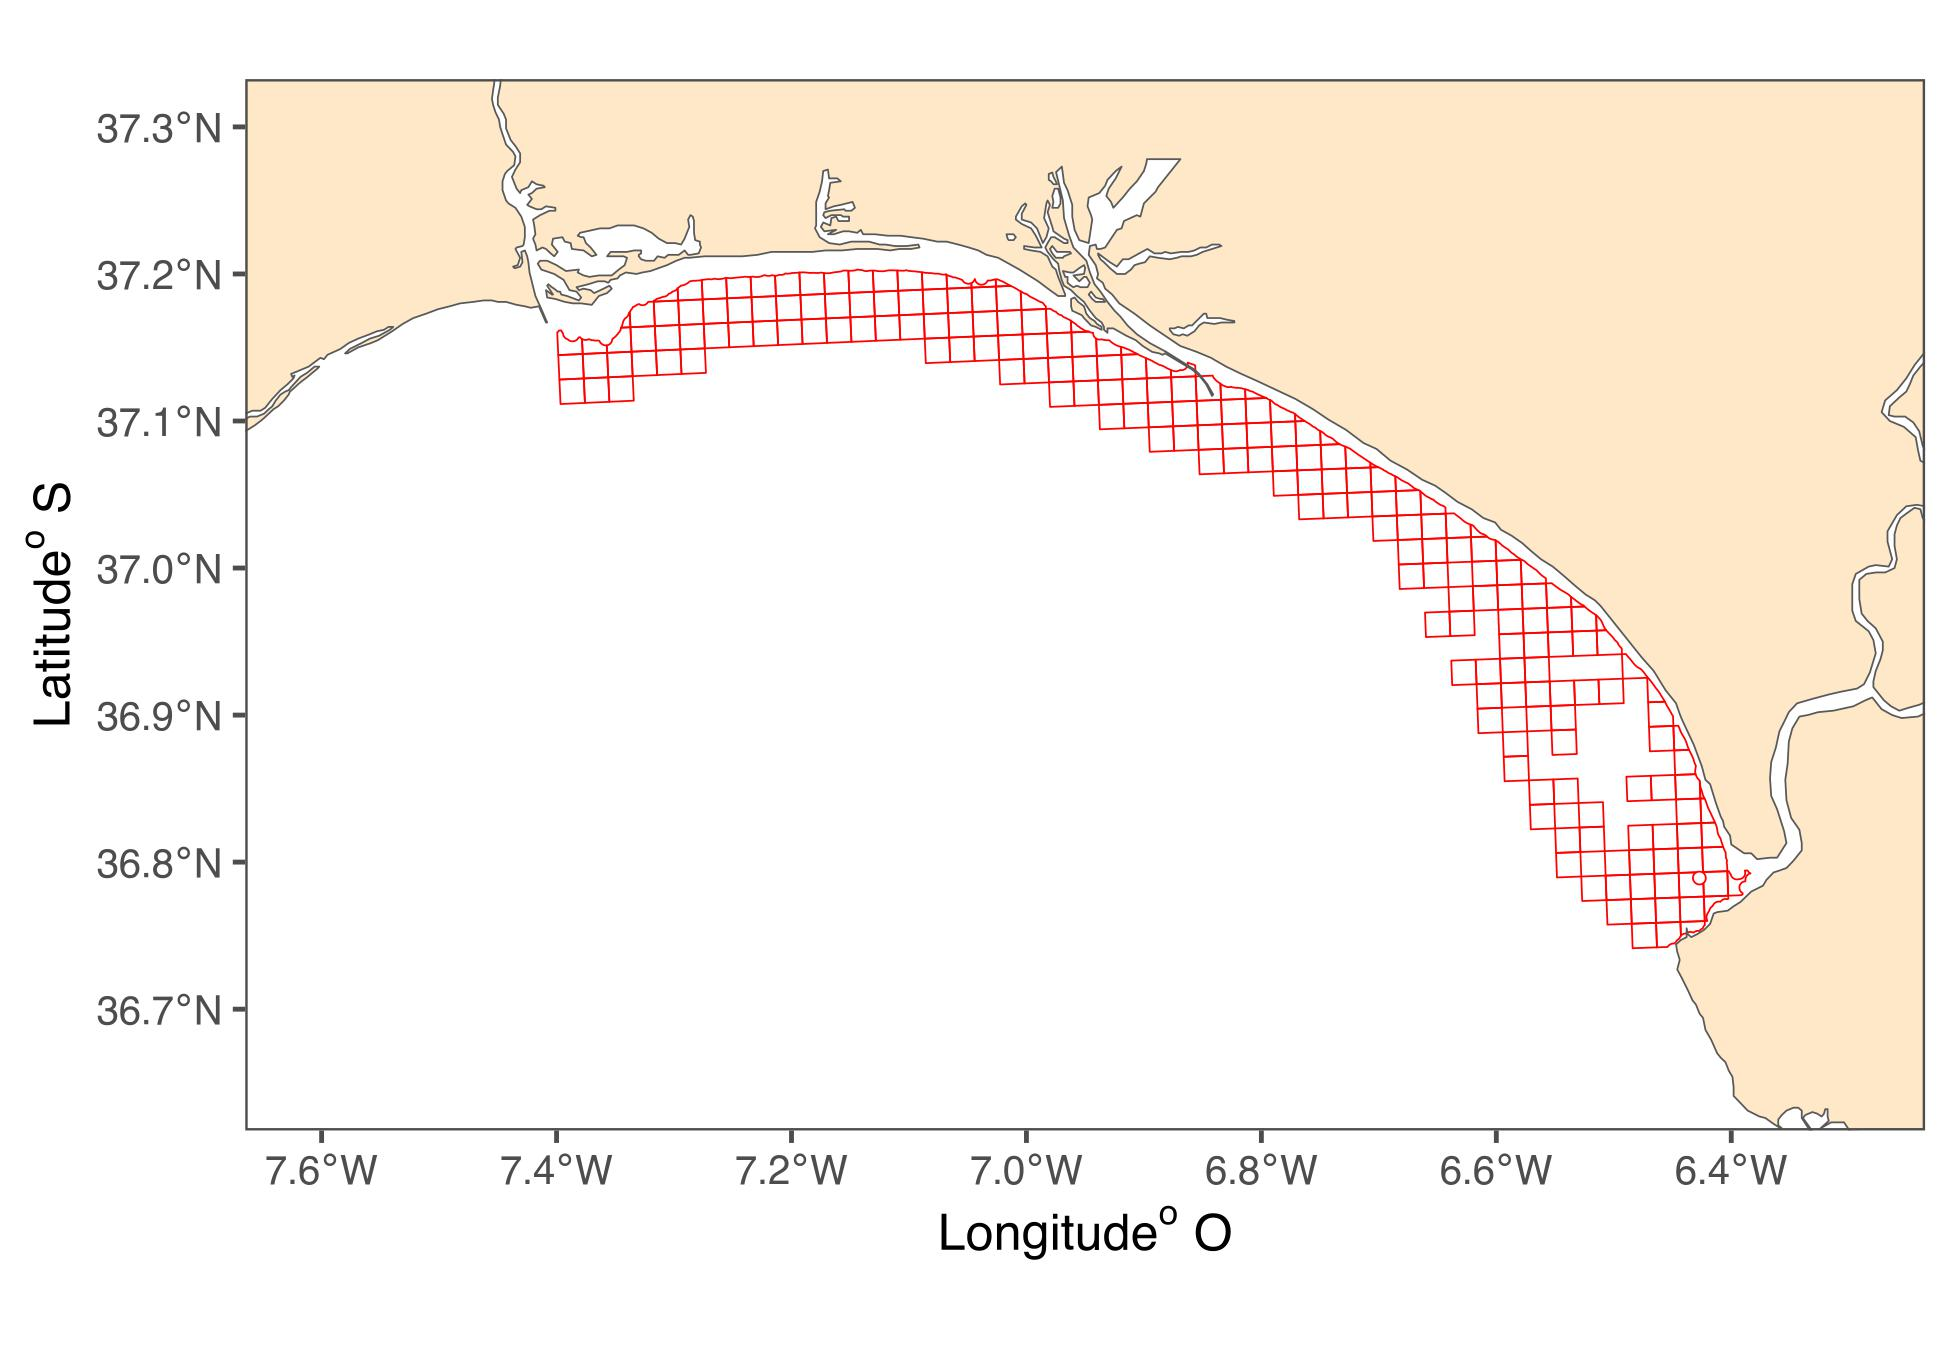
\includegraphics{Habitat_files/figure-latex/unnamed-chunk-3-1} \end{center}

Priebo el mapa

\begin{center}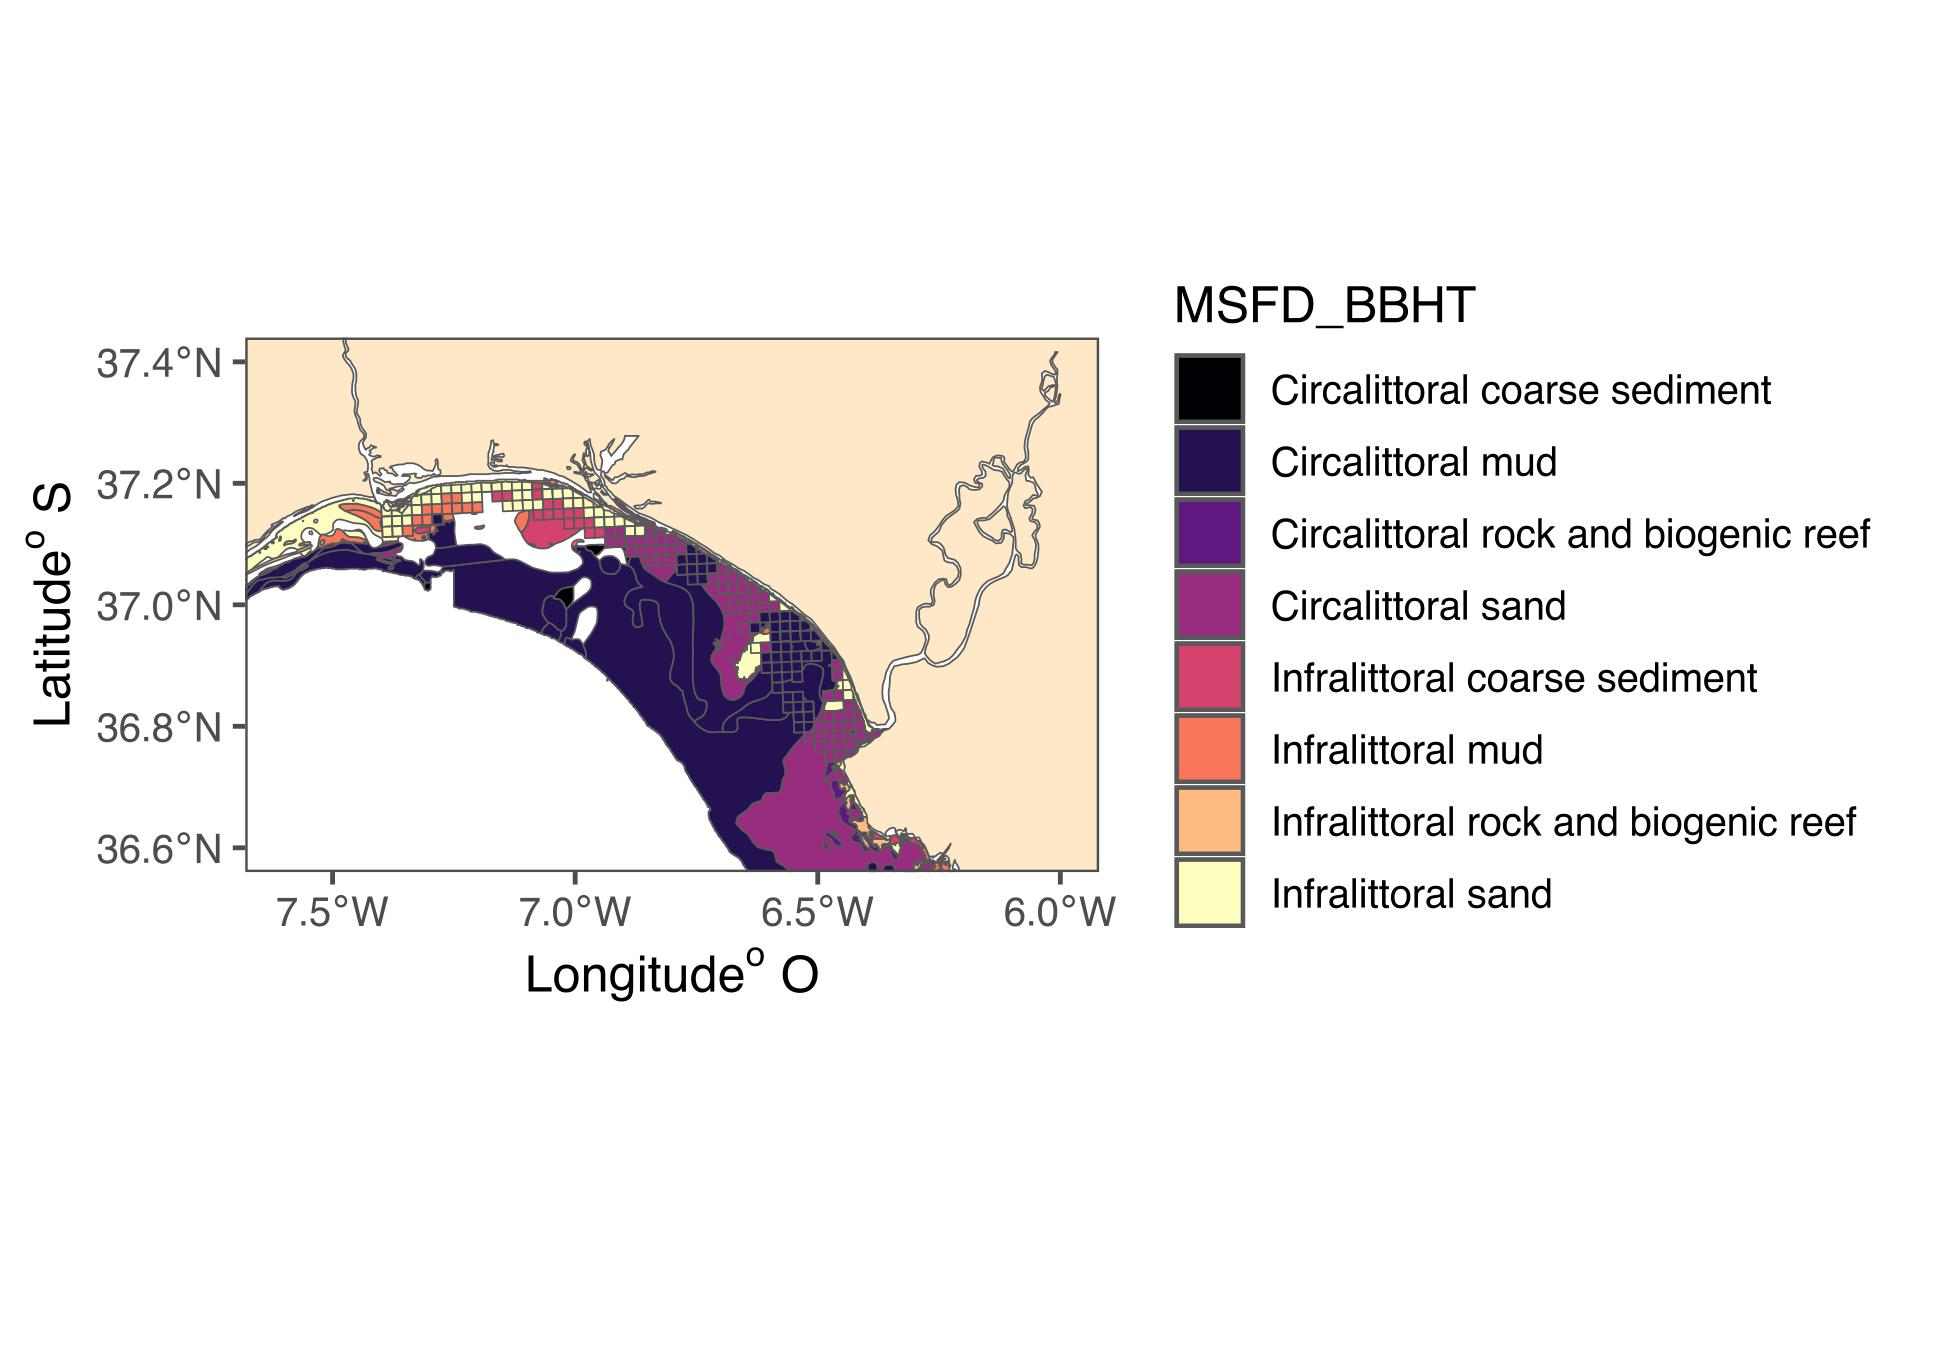
\includegraphics{Habitat_files/figure-latex/unnamed-chunk-4-1} \end{center}

Cuento cuantas estaciones hay por habitat.

\begin{tabular}[t]{l|r}
\hline
Habitat & Nº Estaciones\\
\hline
Circalittoral coarse sediment & 10\\
\hline
Circalittoral mud & 120\\
\hline
Circalittoral rock and biogenic reef & 2\\
\hline
Circalittoral sand & 136\\
\hline
Infralittoral coarse sediment & 37\\
\hline
Infralittoral mud & 134\\
\hline
Infralittoral rock and biogenic reef & 1\\
\hline
Infralittoral sand & 181\\
\hline
NA & 3\\
\hline
\end{tabular}

De acuerdo a esto, ahora unificaré los habitat que consideremos importantes.
La idea es identificar los registros con tiempo efectivo de arrastre como lo muestra la Figura \ref{fig:esq2};

\begin{figure}

{\centering \includegraphics[width=0.5\linewidth]{FIG/diag_habi} 

}

\caption{Esquema para identificar vinculos entre habitats}\label{fig:esq2}
\end{figure}

De acuerdo a esto comenzarmos por juntar los \texttt{Infra} y \texttt{Circa}

ahora veo el mapa

\begin{center}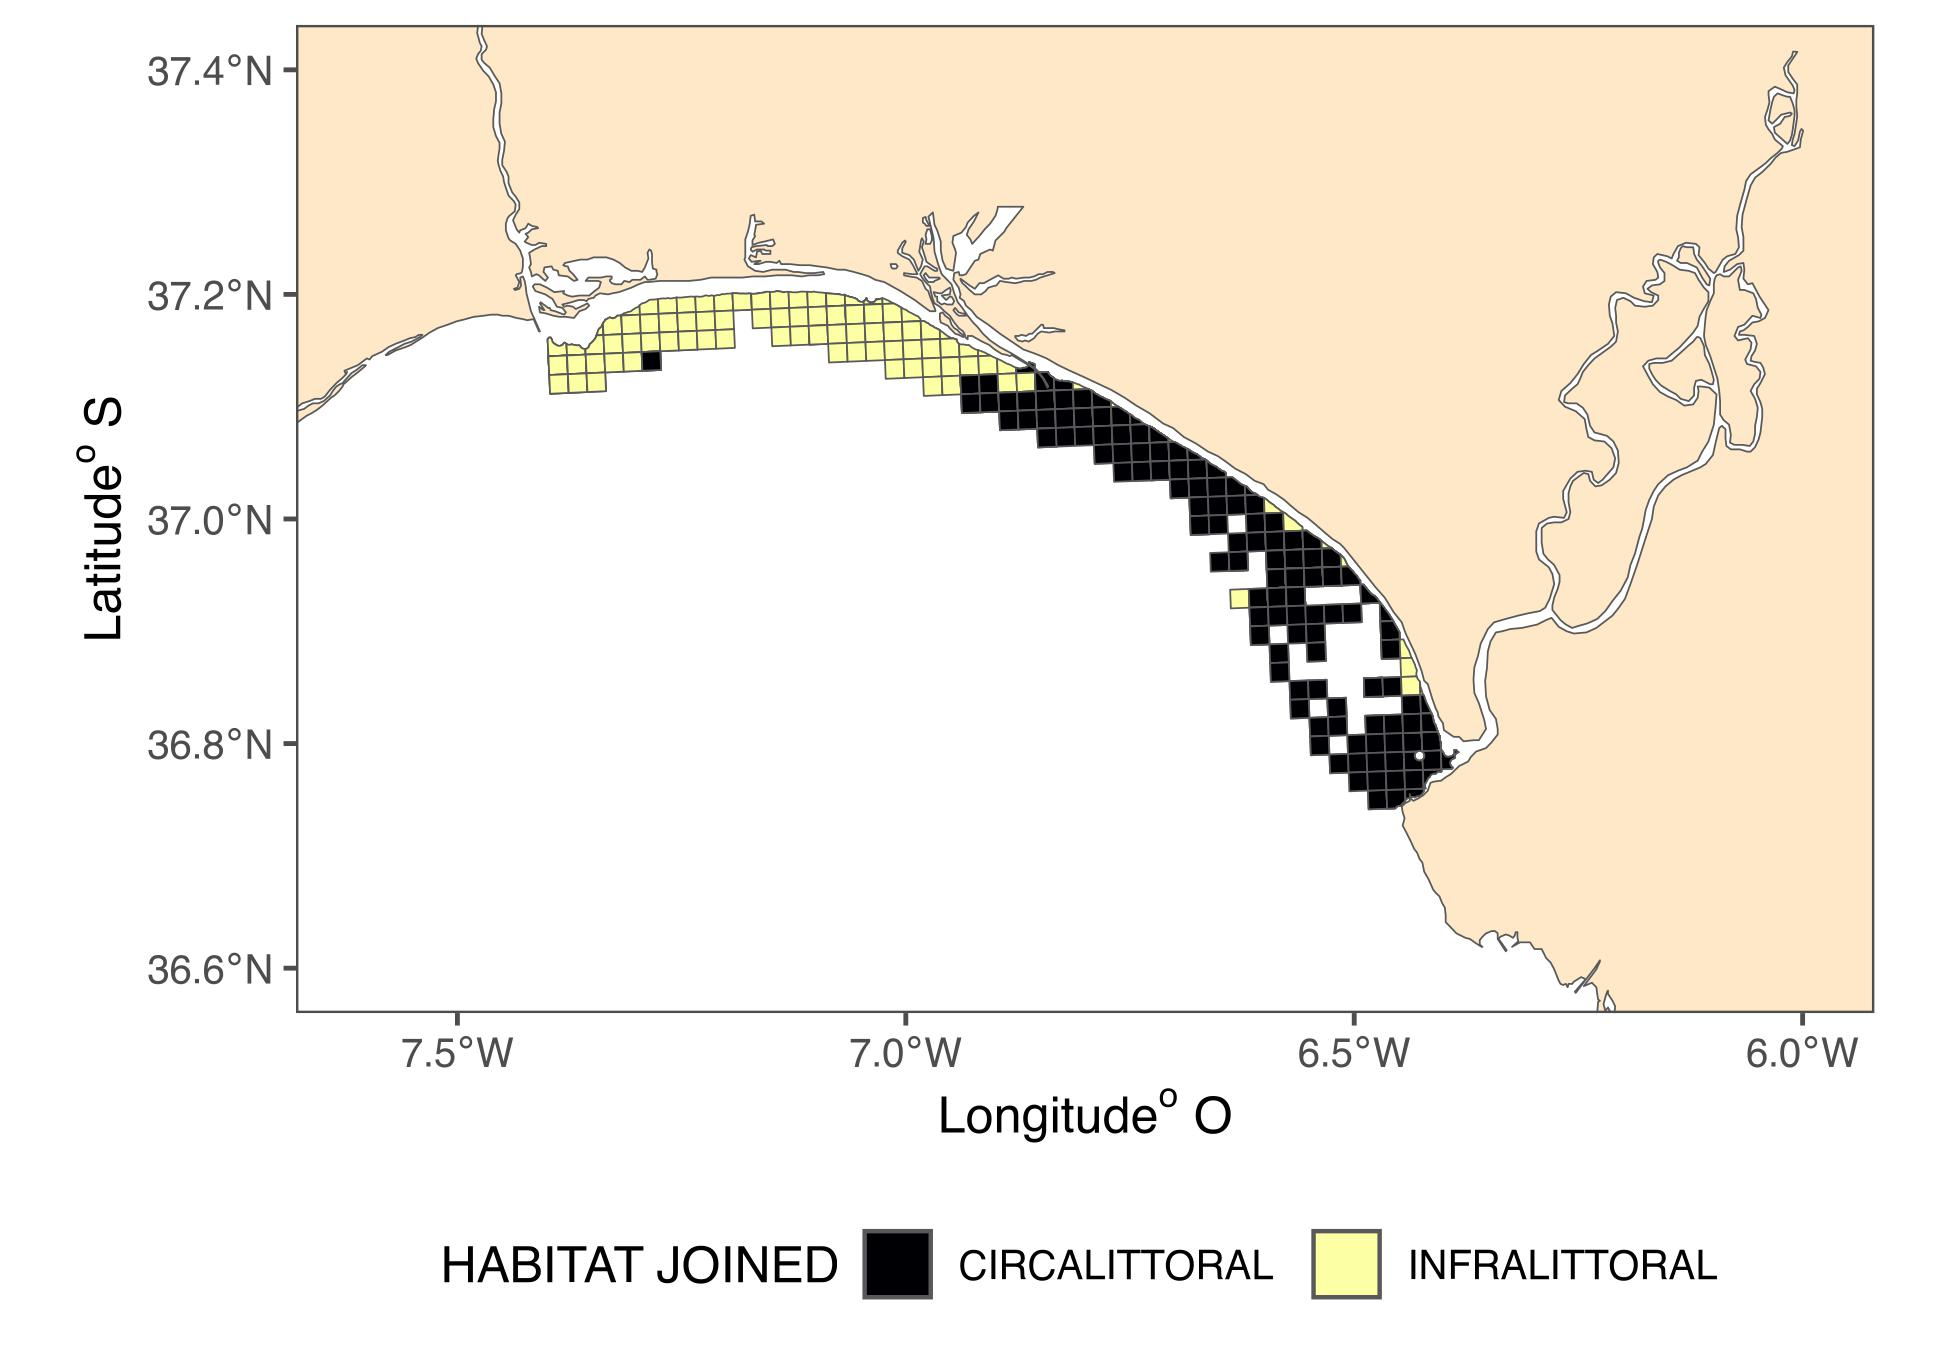
\includegraphics{Habitat_files/figure-latex/unnamed-chunk-7-1} \end{center}

ahora probbar con otro esquema de unir habitats\ldots{}

ahora el mapa 2

ahora veo el mapa

\begin{center}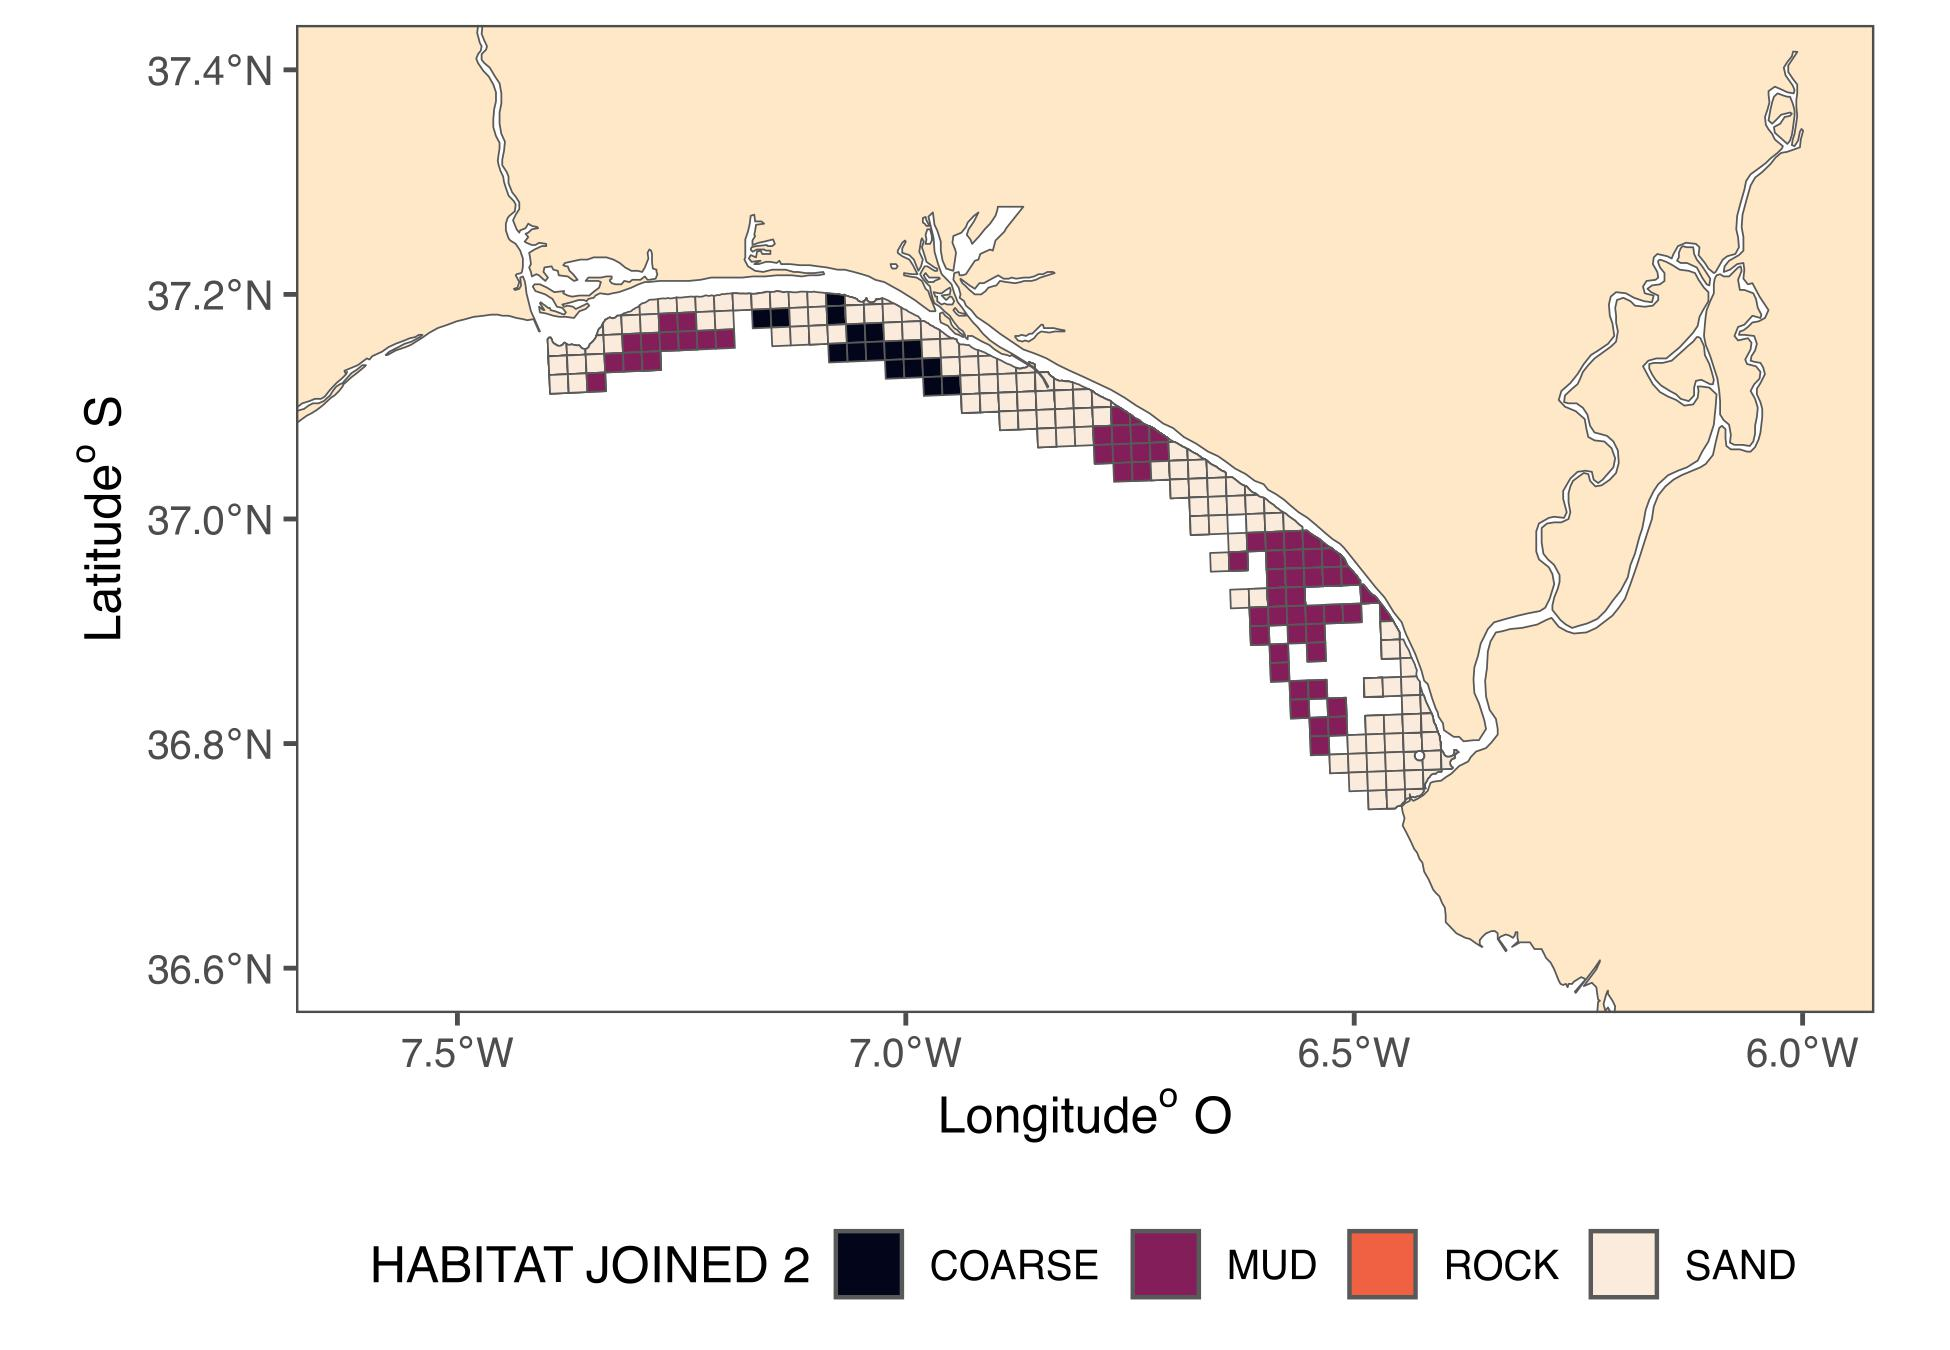
\includegraphics{Habitat_files/figure-latex/unnamed-chunk-9-1} \end{center}

\hypertarget{granulometria}{%
\subsection{Granulometria}\label{granulometria}}

Join grilla

Mapa

\begin{center}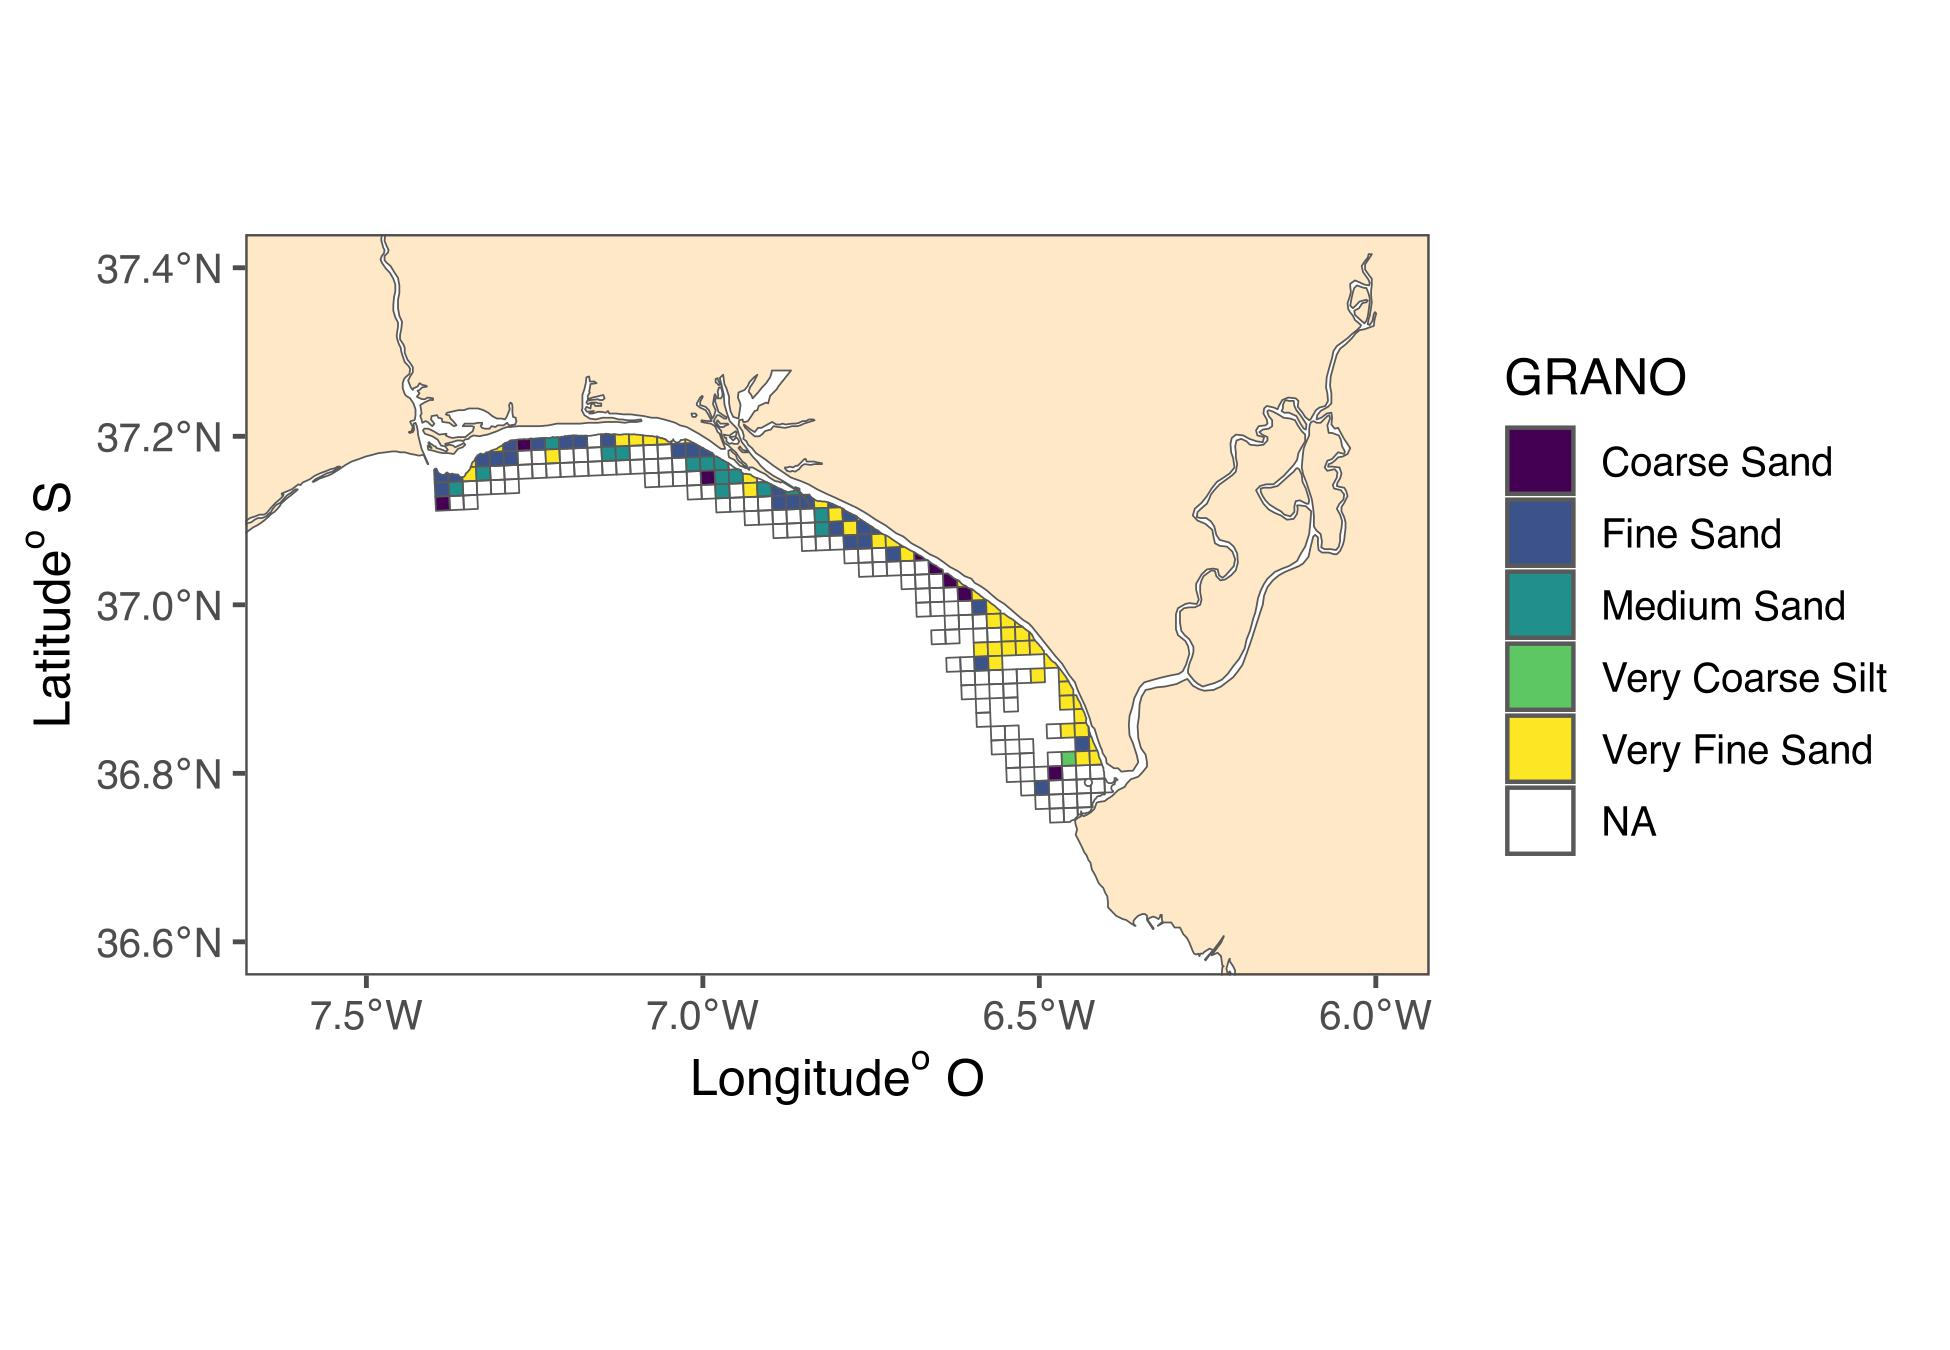
\includegraphics{Habitat_files/figure-latex/unnamed-chunk-12-1} \end{center}

```

\end{document}
